\documentclass[10pt]{article}

\usepackage[margin=0.5in]{geometry}
\usepackage{caption}
\usepackage{color}
\usepackage{colortbl}
\usepackage{graphicx}

\definecolor{red}{rgb}{1,0.85,0.85}
\definecolor{green}{rgb}{0.85,1,0.85}
\graphicspath{{../images/}{../../notebooks/diagrams/}}
\newcommand{\newpar}{\medskip \noindent}

\title{Fingerprinting Automobiles with CAN Bus Data Samples}
\author{David R Crow, 2d Lt, USAF}

\begin{document}
\maketitle

\section{Title}

\newpar Hi, I’m 2d Lt David Crow. My research is about Fingerprinting Vehicles with CAN Bus Data Samples.

\section{Problem Domain}

\newpar Here's a picture of the controller area network \textbf{(citation)}. These are installed in most cars.

\begin{figure}
    \centerline{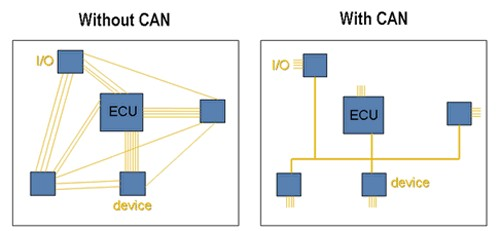
\includegraphics[scale=0.6]{can-wiring.jpg}}
\end{figure}

\newpar Although the CAN clearly reduces system complexity, the network's connectedness means it's a prime target for malicious intruders. If an attacker gains access to the CAN bus through \textit{any} endpoint, they can access the rest of the devices on the network, which include the dashboard, the steering wheel, the brakes, the transmission, the engine, and so on.

\newpar To address this, modern vehicle manufacturers employ a policy of \textit{security through obscurity} when designing the CAN bus and its components. Effectively, this means they make it difficult to interpret the meaning of CAN data without significant reverse engineering efforts. However, this security policy is insufficient for consumer protection because obfuscating a vehicle's CAN data does not adequately hide the vehicle's signature.

\newpar Why is this? Well, today's toolsets can successfully determine whether a specific vehicle generated a specific segment of CAN data, even if said data is unprocessed or limited in scope. This research presents one way to do so.

\section{Objective}

\newpar Specifically, we devise a system capable of identifying which distinct vehicle generated a given segment of CAN bus data. This is a multiclass classification problem which asks the following question: does a given vehicle generate data with some characteristic unique to that vehicle? In other words, does a given vehicle leave identifiable fingerprints on its data?

\newpar We hypothesize that a convolutional neural network can effectively classify vehicles, especially when compared to standard machine learning techniques.

\section{Data}

\newpar This research employs two datasets, one from Oak Ridge National Laboratory and one from a previous student's research \textbf{(citation)}. The lab shared nearly two and a half gigabytes of data captured on the CAN buses of nine different vehicles; Stone captured over 230 megabytes of data from 11 different vehicles.

\begin{table}
    \caption*{Oak Ridge National Laboratory's Vehicles}
    \centering
    \begin{tabular}{|c|c|c|c|}
    \hline
    \textbf{Vehicle} & \textbf{Make} & \textbf{Model} & \textbf{Year} \\
    \hline
    1   & Toyota    & Tacoma    & 2008 \\
    2   & Toyota    & Corolla   & 2009 \\
    3   & Nissan    & Leaf      & 2011 \\
    4   & Ford      & C-Max     & 2013 \\
    5   & Chevrolet & Volt      & 2015 \\
    6   & Ford      & F-150     & 2014 \\
    7   & Ford      & Fusion    & 2016 \\
    8   & Subaru    & WRX       & 2017 \\
    9   & Subaru    & Outback   & 2009 \\
    \hline
    \end{tabular}
\end{table}

\begin{table}
    \caption*{Stone's Vehicles [3]}
    \centering
    \begin{tabular}{|c|c|c|c|}
    \hline
    \textbf{Vehicle} & \textbf{Make} & \textbf{Model} & \textbf{Year} \\
    \hline
    101 & Chevrolet & Cobalt    & 2009 \\
    102 & Chevrolet & Silverado & 2011 \\
    103 & Dodge     & 1500      & 2014 \\
    104 & Ford      & F-150     & 2017 \\
    105 & Ford      & Focus     & 2010 \\
    106 & Honda     & Accord    & 2012 \\
    107 & Honda     & Accord    & 2015 \\
    108 & Nissan    & 370Z      & 2015 \\
    109 & Nissan    & XTERRA    & 2010 \\
    110 & Saab      & 9-7X      & 2009 \\
    111 & Toyota    & Corolla   & 2009 \\
    \hline
    \end{tabular}
\end{table}

\newpar The raw CAN messages in each capture contain a bunch of information. Here's the important stuff:

\begin{table}
    \caption*{Data Samples (Unformatted)}
    \centering
    \begin{tabular}{|c|c|c|l|}
    \hline
    \textbf{Vehicle} & \textbf{Capture} & \textbf{ArbID} & \textbf{Data} \\
    \hline
    3   & 8   & 1532 & \texttt{4A A6 6F FE FF F0 FE}    \\
    3   & 8   & 1532 & \texttt{05 A2 05 A1 05 A2 05 A3} \\
    101 & 101 & 292  & \texttt{FF FF FF FF FF FE FF 00} \\
    108 & 108 & 624  & \texttt{1A 00 41 49 49 40 00 00} \\
    \hline
    \end{tabular}
\end{table}

\newpar Each arb ID might detail a vehicle's speed, RPM, tire pressure, brake pedal position \ldots but we don't actually \textit{know} what it describes. For example, one reverse engineering pipeline might pull these signals from one arb ID. Maybe these are wheel speeds. I don't know. It's impossible to be sure without possessing insider knowledge.

\begin{figure}
    \centerline{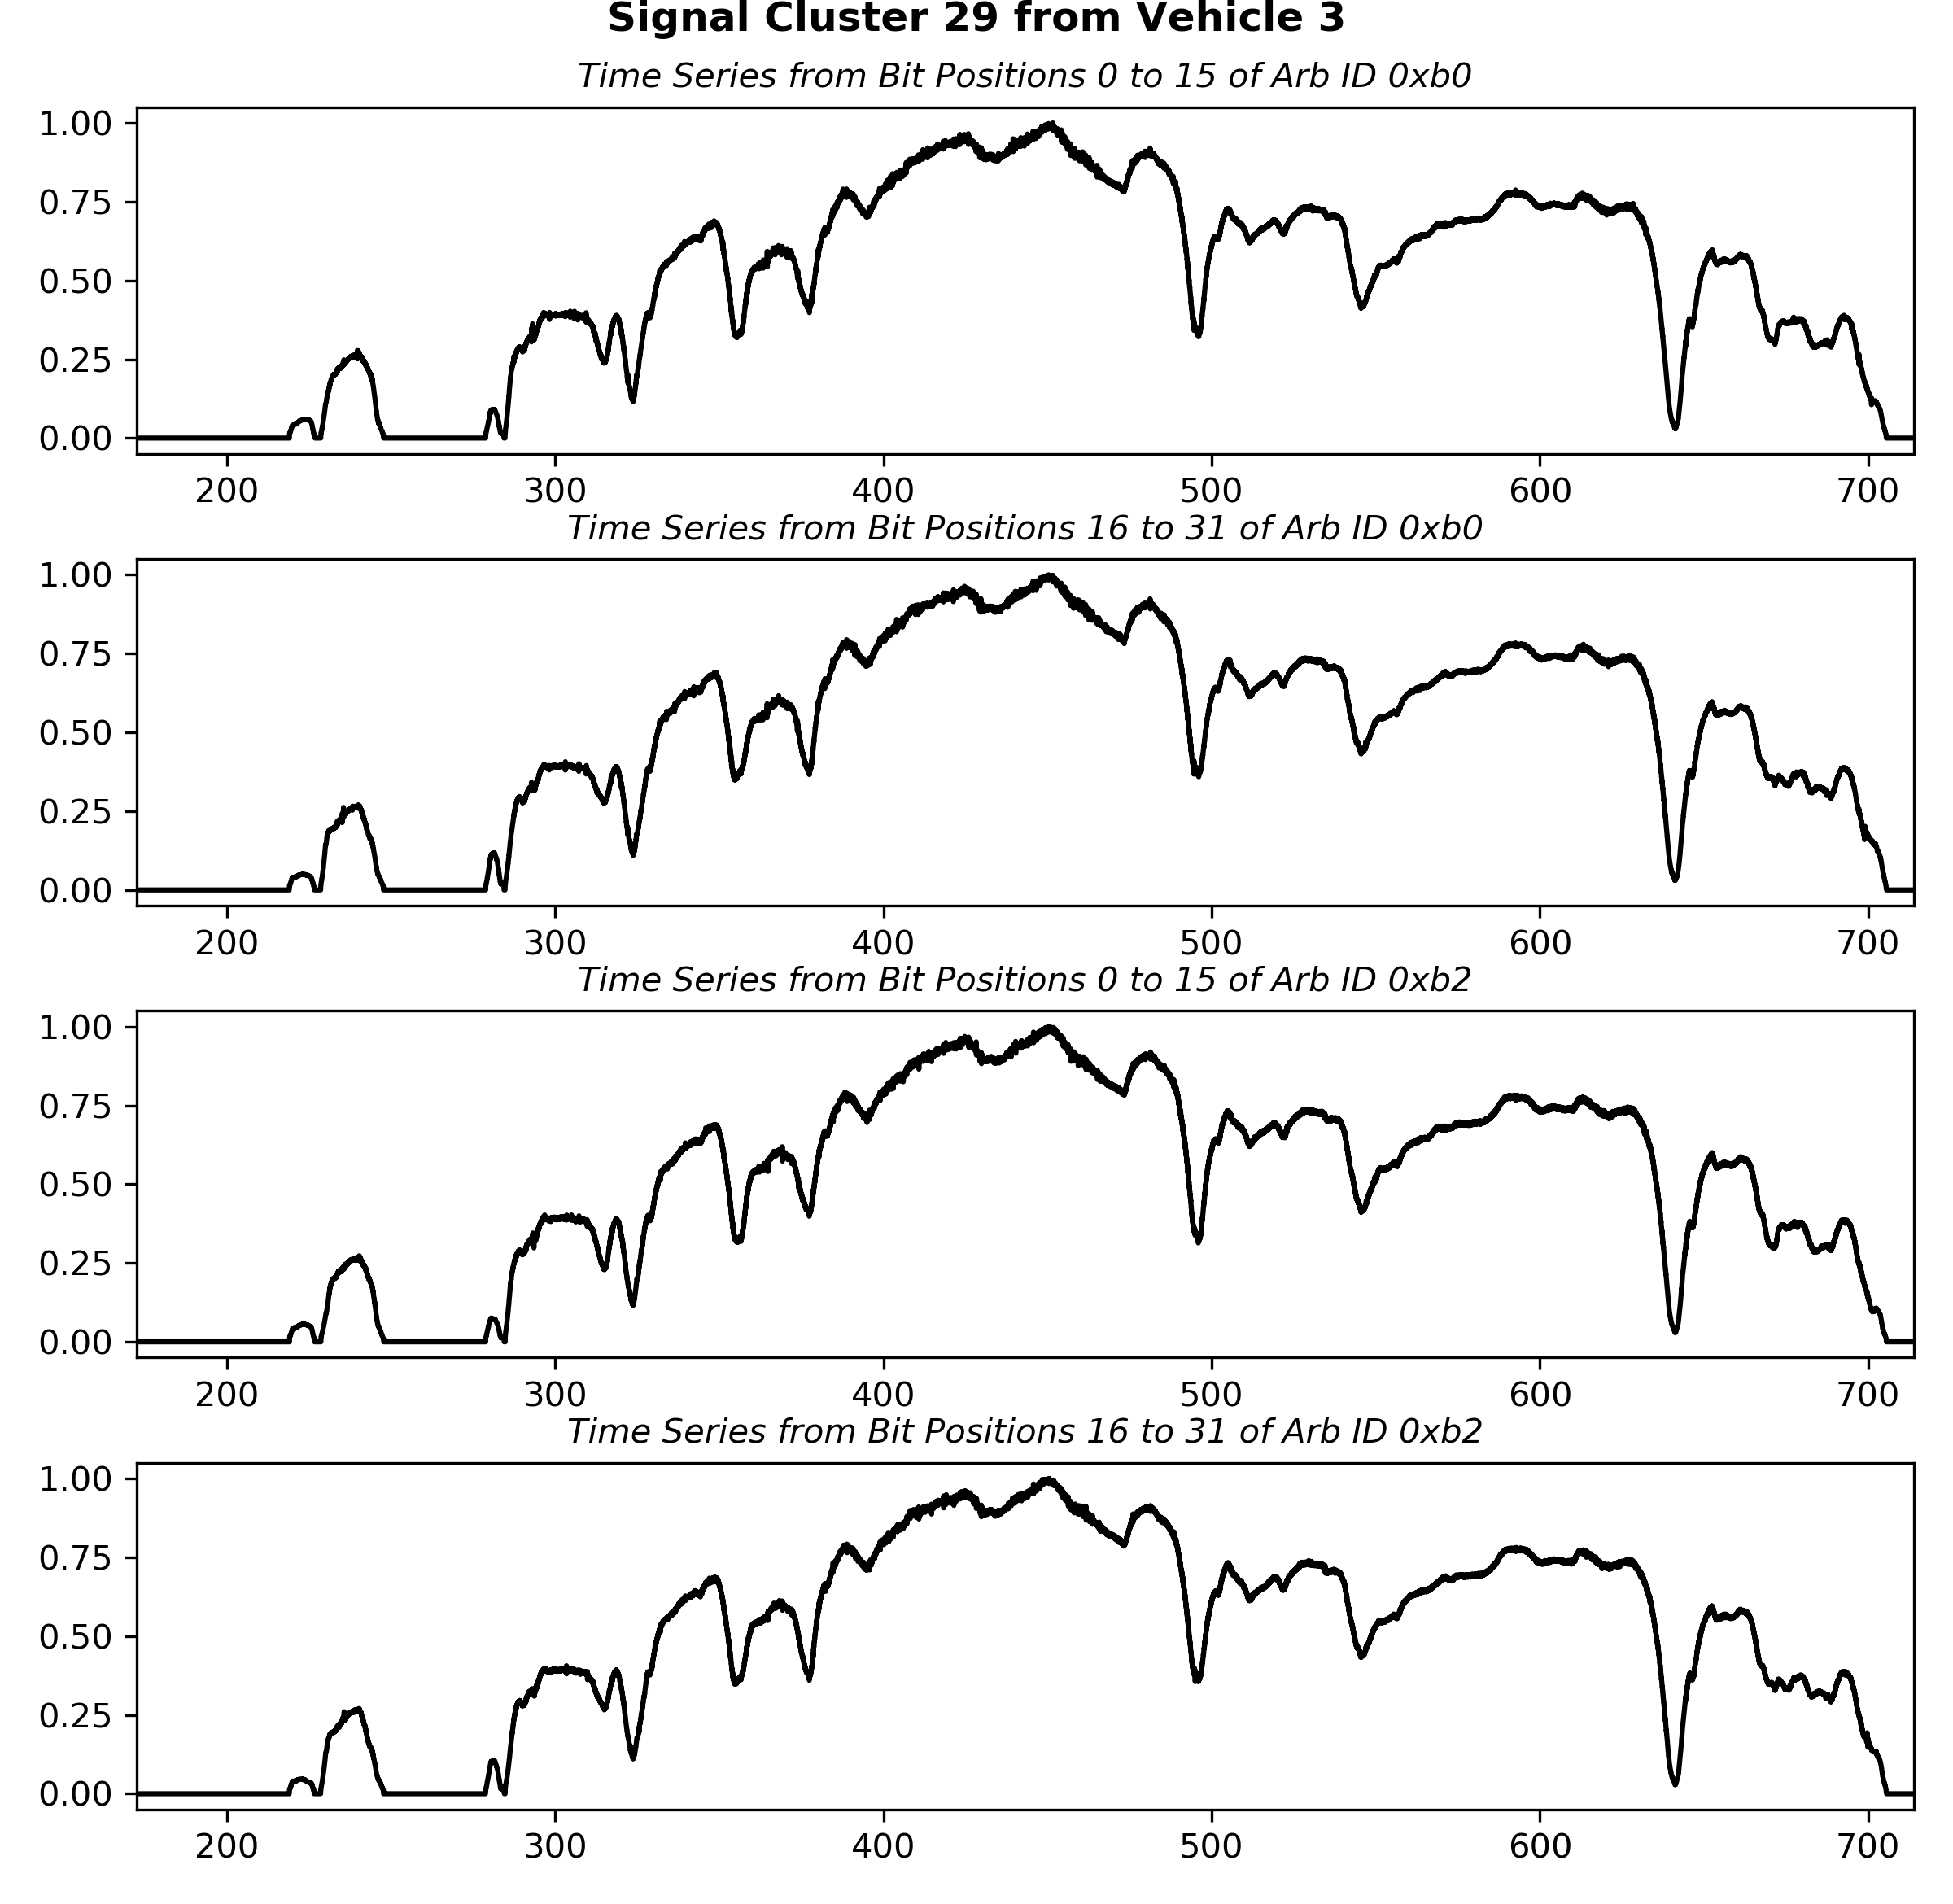
\includegraphics[scale=0.4]{can-signals.png}}
\end{figure}

\newpar Luckily for us, deep learning doesn't particularly care about the meaning of each arb ID. Thus, for every arb ID in every capture, the formatting process entails the following \textbf{(make a nice graphic)}:

\begin{enumerate}
    \item Concatenate all data chunks into one string
    \item Split string into list of hex bytes
    \item Convert list of hex bytes to list of int bytes
    \item Split list of int bytes into list of 1,024-byte samples
    \item Label each sample with generating vehicle (if it's not clear, the task is fully supervised)
\end{enumerate}

\newpar Formatting the datasets in this way gives nearly three hundred thousand samples.

\begin{table}
    \caption*{Data Samples (Formatted)}
    \centering
    \begin{tabular}{|c|c|c|c|}
    \hline
    \textbf{Vehicle} & \textbf{Capture} & \textbf{ArbID} & \textbf{Data} \\
    \hline
    3   & 8   & 1532 & \texttt{074 166 111 254 255 240 254 \ldots} \\
    7   & 24  & 535  & \texttt{003 212 003 209 003 199 003 \ldots} \\
    108 & 108 & 292  & \texttt{255 248 000 128 015 254 030 \ldots} \\
    111 & 111 & 624  & \texttt{026 000 065 073 073 064 000 \ldots} \\
    \hline
    \end{tabular}
\end{table}

\section{Methodology}

\newpar We then train a simple model on 90\% of the data. This simple model is the best version identified in an iterative model-tuning process \textbf{(show model)}. Although it's passable, we can do better \ldots

\newpar \ldots\ So, we also feed these samples into a convolutional neural network. By again looping over model configurations, we identify the best convnet for this task \textbf{(model diagram; parameters; other details)}. This model has about \textbf{(number)} parameters.

\section{Analysis}

\newpar The full dataset is severely imbalanced---Vehicles 3, 5, and 7 are significantly overrepresented, and the remaining vehicles are underrepresented.

\begin{table}
    \caption*{Number of Samples Per Vehicle (Imbalanced)}
    \centering
    \begin{tabular}{|c|r|r|r|r|}
    \hline
    \textbf{Vehicle} & \textbf{Samples} & \textbf{Proportion} \\
    \hline
    1   & 4440   & 1.49  \% \\
    2   & 6895   & 2.32  \% \\
    3   & 141847 & 47.72 \% \\
    4   & 14633  & 4.92  \% \\
    5   & 43377  & 14.59 \% \\
    6   & 9511   & 3.20  \% \\
    7   & 35142  & 11.82 \% \\
    8   & 5018   & 1.69  \% \\
    9   & 8211   & 2.76  \% \\
    101 & 4102   & 1.38  \% \\
    102 & 1824   & 0.61  \% \\
    103 & 1757   & 0.59  \% \\
    104 & 2182   & 0.73  \% \\
    105 & 3791   & 1.28  \% \\
    106 & 1695   & 0.57  \% \\
    107 & 2198   & 0.74  \% \\
    108 & 3020   & 1.02  \% \\
    109 & 2553   & 0.86  \% \\
    110 & 2974   & 1.00  \% \\
    111 & 2083   & 0.70  \% \\
    \hline
    \end{tabular}
\end{table}

\newpar The red rows indicate those classes which are either significantly over- or underrepresented.

\begin{table}
    \caption*{Number of Samples Per Vehicle (Imbalanced)}
    \centering
    \begin{tabular}{|c|r|r|r|r|}
    \hline
    \textbf{Vehicle} & \textbf{Samples} & \textbf{Proportion} \\
    \hline
    \rowcolor{red}
    1   & 4440   & 1.49  \% \\
    \rowcolor{red}
    2   & 6895   & 2.32  \% \\
    \rowcolor{red}
    3   & 141847 & 47.72 \% \\
    4   & 14633  & 4.92  \% \\
    \rowcolor{red}
    5   & 43377  & 14.59 \% \\
    6   & 9511   & 3.20  \% \\
    \rowcolor{red}
    7   & 35142  & 11.82 \% \\
    \rowcolor{red}
    8   & 5018   & 1.69  \% \\
    9   & 8211   & 2.76  \% \\
    \rowcolor{red}
    101 & 4102   & 1.38  \% \\
    \rowcolor{red}
    102 & 1824   & 0.61  \% \\
    \rowcolor{red}
    103 & 1757   & 0.59  \% \\
    \rowcolor{red}
    104 & 2182   & 0.73  \% \\
    \rowcolor{red}
    105 & 3791   & 1.28  \% \\
    \rowcolor{red}
    106 & 1695   & 0.57  \% \\
    \rowcolor{red}
    107 & 2198   & 0.74  \% \\
    \rowcolor{red}
    108 & 3020   & 1.02  \% \\
    \rowcolor{red}
    109 & 2553   & 0.86  \% \\
    \rowcolor{red}
    110 & 2974   & 1.00  \% \\
    \rowcolor{red}
    111 & 2083   & 0.70  \% \\
    \hline
    \end{tabular}
\end{table}

\newpar To address this imbalance, we train on the full dataset and compute balanced accuracy, which accounts for the imbalance. We do the same with a balanced dataset, which we balance by randomly sampling from each of the classes.

\begin{table}
    \caption*{Number of Samples Per Vehicle (Balanced)}
    \centering
    \begin{tabular}{|c|r|r|r|r|}
    \hline
    \textbf{Vehicle} & \textbf{Samples} & \textbf{Proportion} \\
    \hline
    1   & 1695 & 5.00 \% \\
    2   & 1695 & 5.00 \% \\
    3   & 1695 & 5.00 \% \\
    4   & 1695 & 5.00 \% \\
    5   & 1695 & 5.00 \% \\
    6   & 1695 & 5.00 \% \\
    7   & 1695 & 5.00 \% \\
    8   & 1695 & 5.00 \% \\
    9   & 1695 & 5.00 \% \\
    101 & 1695 & 5.00 \% \\
    102 & 1695 & 5.00 \% \\
    103 & 1695 & 5.00 \% \\
    104 & 1695 & 5.00 \% \\
    105 & 1695 & 5.00 \% \\
    106 & 1695 & 5.00 \% \\
    107 & 1695 & 5.00 \% \\
    108 & 1695 & 5.00 \% \\
    109 & 1695 & 5.00 \% \\
    110 & 1695 & 5.00 \% \\
    111 & 1695 & 5.00 \% \\
    \hline
    \end{tabular}
\end{table}

\section{Results}

% todo: What were your results? Show some graphs/tables/figures and describe them.

\newpar Results indicate that the simple model can adequately classify vehicles, but it's clear that the convnet is a bit better.

\begin{table}
    \caption*{Balanced Accuracy for Each Model}
    \centering
    \begin{tabular}{|c|c|c|}
    \hline
    \textbf{Model} & \textbf{Dataset} & \textbf{Accuracy} \\
    \hline
    Multi-layer perceptron       & Imbalanced & 81.71 \% \\
    Multi-layer perceptron       & Balanced   & 76.95 \% \\
    Convolutional neural network & Imbalanced & 83.18 \% \\
    Convolutional neural network & Balanced   & 80.94 \% \\
    \hline
    \end{tabular}
\end{table}

\begin{table}
    \caption*{Best and Worst Vehicles for Each Model}
    \centering
    \begin{tabular}{|c|c|c|c|}
    \hline
    \textbf{Model} & \textbf{Dataset} & \textbf{Best Vehicle} & \textbf{Worst Vehicle} \\
    \hline
    MLP & Imbalanced & 1   & 111 \\
    MLP & Balanced   & 6   & 105 \\
    CNN & Imbalanced & 9   & 102 \\
    CNN & Balanced   & 105 & 7   \\
    \hline
    \end{tabular}
\end{table}

\begin{table}
    \caption*{Class Accuracy for Each Vehicle}
    \centering
    \begin{tabular}{|c|c|c|c|c|c|}
    \hline
    \textbf{Vehicle} & \textbf{MLP Imbalanced} & \textbf{MLP Balanced} & \textbf{CNN Imbalanced} & \textbf{CNN Balanced} & \textbf{Median} \\
    \hline
    1 & \cellcolor{green}98.31 \% & \cellcolor{red}83.29 \% & 92.58 \% & 88.20 \% & 90.39 \\
    2 & 86.89 \% & \cellcolor{red}76.61 \% & \cellcolor{green}88.69 \% & 80.88 \% & 83.88 \\
    3 & 93.59 \% & 81.82 \% & \cellcolor{green}93.60 \% & \cellcolor{red}74.21 \% & 87.70 \\
    4 & 94.40 \% & \cellcolor{red}76.52 \% & \cellcolor{green}94.55 \% & 77.87 \% & 86.13 \\
    5 & 96.85 \% & \cellcolor{red}70.72 \% & \cellcolor{green}97.56 \% & 81.57 \% & 89.21 \\
    6 & \cellcolor{green}96.20 \% & 94.72 \% & 94.72 \% & \cellcolor{red}83.63 \% & 94.72 \\
    7 & 89.50 \% & 70.47 \% & \cellcolor{green}92.71 \% & \cellcolor{red}48.27 \% & 79.98 \\
    8 & 94.99 \% & 92.49 \% & \cellcolor{green}96.85 \% & \cellcolor{red}89.34 \% & 93.74 \\
    9 & 96.03 \% & \cellcolor{red}86.26 \% & \cellcolor{green}98.34 \% & 92.64 \% & 94.33 \\
    101 & 87.54 \% & \cellcolor{red}60.22 \% & \cellcolor{green}89.00 \% & 83.38 \% & 85.46 \\
    102 & \cellcolor{green}97.63 \% & 84.31 \% & 82.51 \% & \cellcolor{red}75.56 \% & 83.41 \\
    103 & 85.67 \% & 89.51 \% & \cellcolor{green}93.57 \% & \cellcolor{red}81.59 \% & 87.59 \\
    104 & \cellcolor{red}83.18 \% & \cellcolor{green}89.55 \% & 89.29 \% & 87.83 \% & 88.56 \\
    105 & 91.80 \% & \cellcolor{red}50.83 \% & 93.94 \% & \cellcolor{green}94.83 \% & 92.87 \\
    106 & 89.38 \% & \cellcolor{green}89.70 \% & 85.59 \% & \cellcolor{red}85.17 \% & 87.48 \\
    107 & 82.52 \% & \cellcolor{red}69.44 \% & \cellcolor{green}87.41 \% & 79.26 \% & 80.89 \\
    108 & 94.42 \% & \cellcolor{red}73.61 \% & \cellcolor{green}95.12 \% & 89.64 \% & 92.03 \\
    109 & 90.79 \% & 85.71 \% & \cellcolor{green}93.60 \% & \cellcolor{red}82.67 \% & 88.25 \\
    110 & \cellcolor{red}82.18 \% & 84.50 \% & 83.78 \% & \cellcolor{green}87.81 \% & 84.14 \\
    111 & 74.01 \% & \cellcolor{red}70.98 \% & \cellcolor{green}88.07 \% & 78.80 \% & 76.40 \\
    \hline
    N/A & 81.71 \% & 76.95 \% & 83.18 \% & 80.94 \% & N/A \\
    \hline
    \end{tabular}
\end{table}

\section{Impacts \& Limitations}

% todo: What are the impacts of your results, and what assumptions/limitations are there with your results?

\section{Future Work}

\newpar Devising a siamese neural network capable of learning the difference between CAN segments is the logical next step for this research. As a reminder, an SNN can generalize to new classes because it learns why two observations come from the same class or from different classes. A standard CNN, on the other hand, must learn every class. For this reason, an SNN is extensible: one can train an SNN on a set of vehicles and, because it knows why samples from two vehicles are different, one can introduce new vehicles and still maintain solid performance.

\begin{figure}
    \centerline{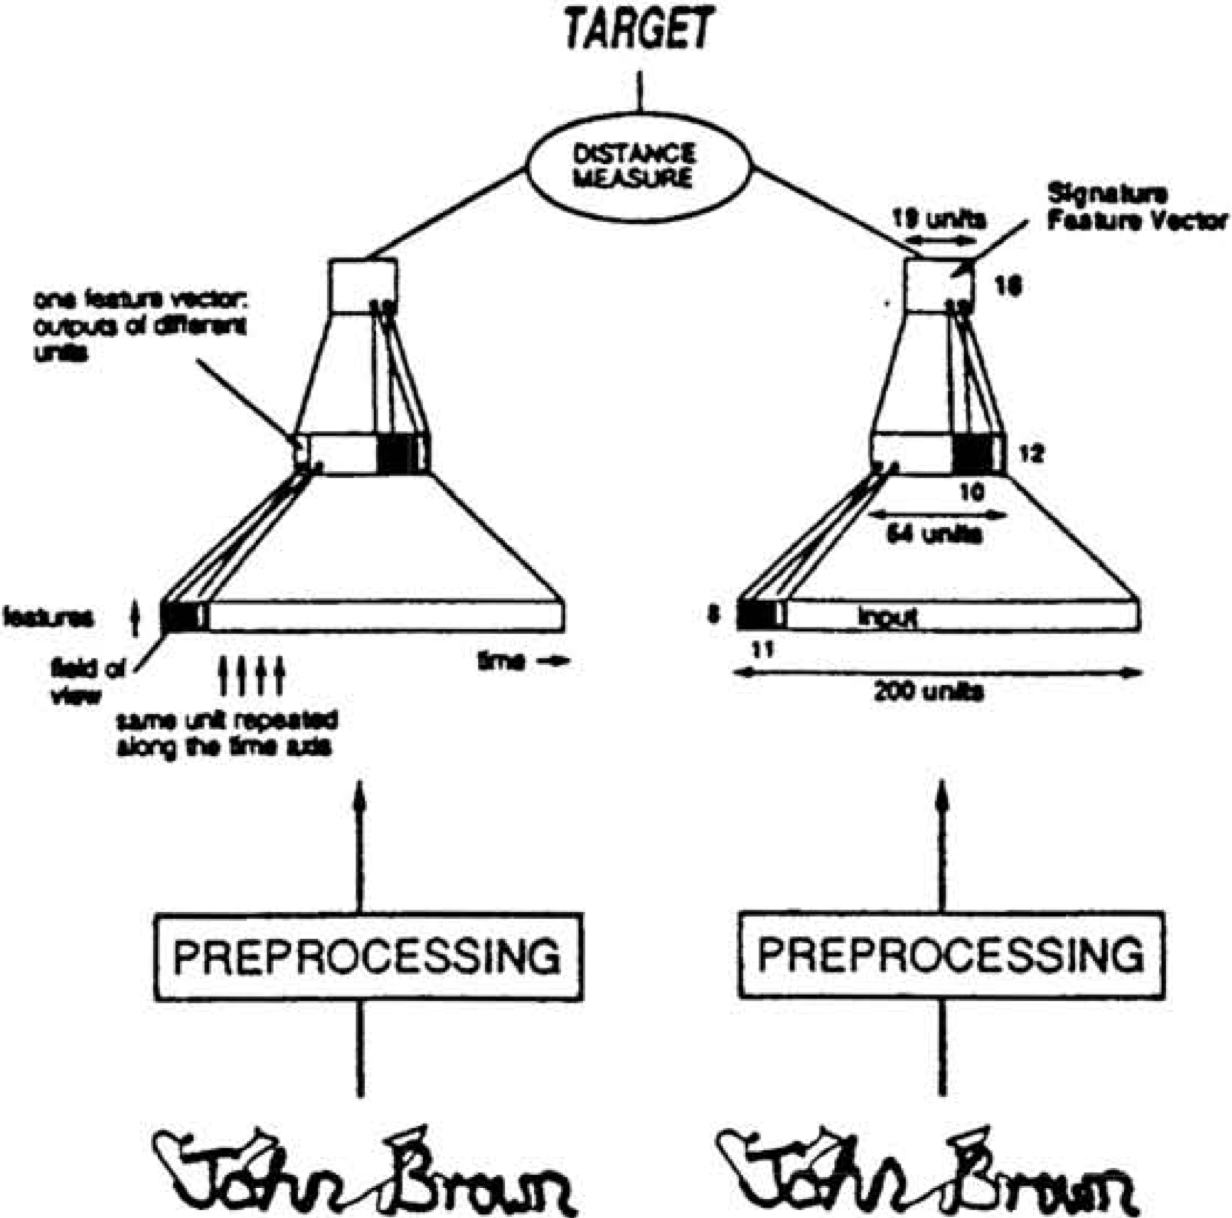
\includegraphics[scale=0.5]{snn.png}}
\end{figure}

\section{References}

\newpar Here are some references \dots

\section{Thank You}

\newpar \ldots\ And thanks for watching. Let me know if you have any questions!

\end{document}
